\section[Měření rozložení hustoty toku]{Měření rozložení hustoty toku neutronů a jejich spektra v aktivní zóně reaktoru}

Detailní znalost rozložení hustoty toku neutronů v AZ je nutná jak z pohledu bezpečného, tak i optimálního provozu jaderného reaktoru (energetického i výzkumného, např. při využívání paliva). V případě výzkumných reaktorů je tato znalost důležitá pro přípravu experimentů (především ozařovacích). Hustota toku neutronů je funkcí závislou jak na poloze v AZ reaktoru, tak i energii neutronů, jelikož v reaktoru se nacházejí neutrony všech energií od maximálních hodnot spektra po spektrum tepelné. Pro správnou interpretaci výsledků experimentů je nutné, aby rozložení hustoty toku neutronů bylo zmapováno nejen jako funkce polohy, ale i energie neutronů.

Obvykle jsou prováděny dva typy experimentů, které souvisejí s měřením hustoty toku neutronů:

\begin{itemize}%[noitemsep]
    \item[$-$] měření relativního rozložení hustoty toku neutronů v axiálním i radiálním směru,
    \item[$-$] určení absolutní hustoty toku neutronů.
\end{itemize}

Relativní rozložení hustoty toku neutronů lze získat z měření s malými aktivačními detektory ve formě folií (nebo drátů), či pomocí plynových detektorů s malými aktivními rozměry. V případě reaktorů s dostatečně vysokým výkonem lze k rozložení hustoty toku neutronů použít také samonapájecí detektory. Určování absolutní velikosti hustoty toku neutronů se provádí obvykle pomocí vhodného aktivačního detektoru (nejčastěji tenká folie zlata). Hrubého energetického rozdělení na tepelné a epitermální neutrony lze docílit pokrytím detektorů kadmiem.

\subsection{Axilální rozložení hustoty toku neutronů}

\subsubsection{Rozložení dle difúzní teorie}

Chceme-li získat analytické řešení popisující axiální rozložení hustoty toku neutronů v jaderném reaktoru, je nutné použít řadu zjednodušení, která se týkají jak sledované energie neutronů, tak i zvoleného geometrického uspořádání reaktoru. Nejjednodušším přiblížením je difuzní model založený na jednoskupinové teorii neutronů. V tomto případě předpokládáme, že neutrony vznikají, difundují a jsou absorbovány při jedné energii, a to energii tepelné. Tento model můžeme použít k popisu rozložení hustoty toku neutronů v AZ homogenního reaktoru bez reflektorů, pomocí stacionární difuzní rovnice ve tvaru:

\begin{equation*}
D \cdot \nabla^2 \phi - \Sigma_{a} \cdot \phi + \dfrac{1}{k} \cdot \Sigma_{f} \phi \nu= 0
\end{equation*}

kde:

\begin{itemize}
    \item[$-$] $D$ je difuzní koeficient v AZ,
    \item[$-$] $\phi$ je hustota toku neutronů v AZ,
    \item[$-$] $\Sigma_{a}$, $\Sigma_{f}$ je makroskopický účinný průřez pro absorpci, štěpení v AZ,
    \item[$-$] $\nu$ je průměrný výtěžek neutronů ze štěpení,
    \item[$-$] $k$ je koeficient násobení.
\end{itemize}

Zavedením geometrického faktoru $B^2$ a vyřešením difuzní rovnice s okrajovými podmínkami, dostáváme tvar:

\begin{equation}
    \phi = A \cdot \cos{\left(\dfrac{\pi z}{H'}\right)}
\end{equation}

Složitější situace nastává, pokud chceme popsat axiální rozložení hustoty toku neutronů v AZ s reflektorem. Účelem reflektoru je vracet zpět do AZ unikající neutrony, které by byly jinak pro štěpnou řetězovou reakci ztracené. Tím, že se sníží únik neutronů ze soustavy, můžeme při stejném složení AZ dosáhnout podstatně menších kritických rozměrů, než jsou potřebné pro reaktor bez reflektoru. Kromě tohoto efektu způsobuje reflektor zvýšení specifického výkonu reaktoru tím, že se v periferní oblasti AZ zvyšuje hustota toku neutronů a i průměrná hustota toku v celé aktivní oblasti. TOmuto nárůstu v hustotě toku se říká reflektorové peaky.

V případě popisu rozložení hustoty toku neutronů v AZ s reflektorem je nutné použít dvouskupinovou teorii. Jednoskupinová teorie předpokládá, že všechny neutrony jsou tepelné a nezahrnuje skutečnost, že u rychlých neutronů unikajících do reflektoru, je větší pravděpodobnost, že budou rozptýleny zpět do AZ při srážkách, ke kterým dojde při zpomalení. Navíc neutrony, které vnikají do reflektoru s nad-rezonančními energiemi, se v reflektoru zpomalují a mohou se vrátit do AZ jako neutrony tepelné. Tím by se zcela vyhnuly rezonančnímu zachycení v palivu, které by nastalo, kdyby se zpomalovaly v AZ reaktoru. Tyto okolnosti zvyšují účinnost reflektoru ve srovnání s jeho účinností, jakou by měl reflektor, kdyby všechny neutrony byly tepelné.

\begin{figure}[H]
    \centering
    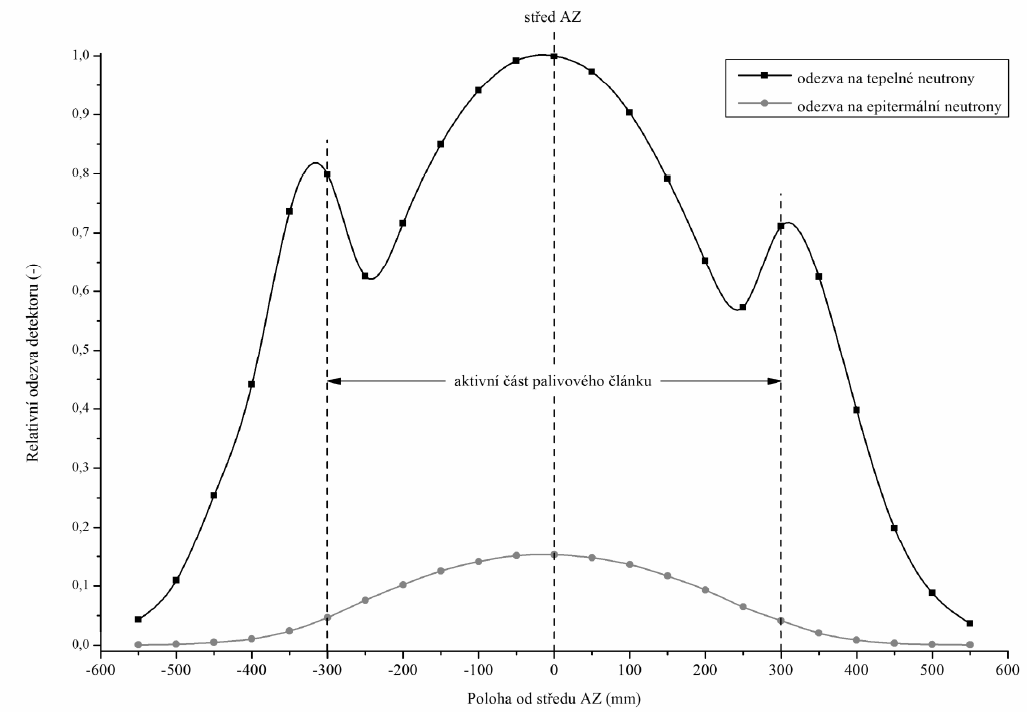
\includegraphics[scale=0.6]{img/AxiálníRozloženíVýkonu.png}
    \caption{Axiální rozložení výkonu s reflektorem.}
    \label{fig:AxiálníRozložníVýkonu}
\end{figure}

\subsubsection{Měření rozložení hustoty toku neutronů plynovými detektory}

Jeden ze způsobů experimentálního stanovení rozložení hustoty toku tepelných neutronů je využití rozměrově malých plynových detektorů pracujících v impulsním režimu. Obvykle se jedná o detektory plněné $^3$He nebo detektory s konvertorem neutronů v podobě tenké vrstvy z vysoce obohaceného $^{10}$B. Tyto detektory se umisťují do suchých vertikálních kanálů v AZ, kde na základě jejich odezvy (četnost $CR$) můžeme získat informaci o poli neutronů v AZ nebo její periferii. V případě postupného protahování detektoru po výšce kanálu obdržíme axiální rozložení hustoty toku neutronů.

Při vysouvání detektoru z AZ může docházet ke zkreslení jeho odezvy, jelikož detektor prochází od oblastí s minimálními hustotami toku neutronů (vně AZ) do oblastí maximálních hustot toku neutronů (střed AZ). V takovém případě je nutné provést korekci na nelinearitu odezvy detektoru tak, abychom získali její nezkreslenou hodnotu. Nelinearita je způsobena především mrtvou dobou detekčního systému. Jednou z metod, které se používá k určení korekčního činitele nelinearity, respektive mrtvé doby detekčního systému, je metoda srovnání detekčního systému, který je v celém rozsahu měřicích četností lineární. Vhodným detekčním systémem pro tyto účely je kompenzovaná ionizační komora pracující v proudovém režimu pro měření malých proudů. Kompenzace zajišťuje korekce odezvy a srovnávací měření této komory již umožňuje zjistit lineární odezvu detekčního systému i pro vysoké hustoty toku neutronů.

\subsubsection{Měření rozložení hustoty toku neutronů samonapájecími detektory}

Samonapájecí detektory se využívají převážně v energetických reaktorech. Skládají se z tenkého drátku s velkým účinným průřezem pro záchyt neutronů, který vede k produkci $\beta^-$ nestabilního izotopu s kratším poločasem rozpadu (typicky rhodium nebo vanad). Tento drátek je obalen vrstvou izolantu, na kterou navazuje vodivý materiál kolektoru, který snímá impulzy. $\beta^-$ nestabilní izotop se ustaluje do rovnovážné koncentrace, která je úměrná absolutní hustotě toku neutronů v daném místě. Následně se rozpadá a vzniklé elektrony putují do kolektoru, kde jsou snímány jako elektrický proud ($\beta^-$ částice jsou v podstatě elektrony, které zapřičiňují vznik a přesun náboje v kolektoru).

Jejich výhoda spočívá v tom, že nepotřebují napájení a pro každý detektor stačí pouze jeden drátek jako vývod do měřícího počítače. Zároveň jsou malé a skladné, do centrální trubice palivového souboru se jich naskládá několik, čímž je možné získat axiální rozložení neutronů v daném souboru.

\subsubsection{Měření rozložení hustoty toku neutronů aktivačními detektory}

Aktivační detektory lze úspěšně použít také k určování prostorového rozložení hustoty toku neutronů v AZ. Jejich výhodou jsou malé rozměry a možnost je umístit do oblastí, ve kterých nelze použít elektronické detektory. Nevýhodou naopak je, že tím nezískáme on-line monitoring a rozložení zjistíme až zpětným měřením.

Vhodnou volbou aktivačního materiálu nebo jeho kombinace s filtry neutronů lze měřit neutrony z různých energetických oblastí. Pro měření rozložení hustoty toku neutronů můžeme využít aktivační detektory ve tvaru malé tenké fólie, respektive sady fólií. Ještě lepší je použít drátek, který protáhnu axiálně celým reaktorem, ozářím, a pro následné měření rozstříhám. Nejčastěji používanými materiály pro výrobu aktivačních detektorů ve tvaru drátu, které jsou citlivé především na tepelné, respektive epitermální neutrony, jsou zlato, měď nebo dysprosium.

Zlato je vhodným materiálem pro zhotovení aktivačních detektorů jak z důvodů mechanických, tak i fyzikálních vlastností. Jeho určitou nevýhodou je vyšší pořizovací cena. Zlato se velmi často používá pro absolutní měření hustoty toku neutronů, protože má velmi přesně stanovenou hodnotu účinného průřezu a poločasu rozpadu. Poločas rozpadu je dostatečně dlouhý pro přenos i analýzu ozářených aktivačních detektorů na detekčním systému. Účinný průřez izotopu zlata $^{197}$Au (v přírodě 100 \% zastoupení) pro radiační záchyt neutronu se v oblasti tepelných neutronů řídí zákonem 1/v, jelikož jeho první výrazná rezonance leží již na energii $E_n = 4{,}9 \, \text{eV}$. Proto se zlato používá nejen pro měření tepelných, ale i epitermálních neutronů. Často se používá ve slitinách s jinými prvky, např. s hliníkem.

\begin{equation*}
    ^{198}\text{Au} \xrightarrow{T_{1/2} = 2,69\ d}\ ^{198}\text{Hg} + e^- + \gamma.
\end{equation*}

Tímto rozpadem vzniká gamma peak na energii $E_\gamma = 411,8$ keV s intenzitou $I_\gamma = 96\ \%$.

Následné zpětné určení hustoty toku je založeno na určování reakční rychlosti ($RR$). S využitím kadmiového pouzdra lze měřit reakční rychlost epitermálních neutronů ($RR_\text{Cd}$). Reakční rychlost od tepelných neutronů lze poté stanovit podle vzorce:

\begin{equation*}
    RR_\text{th} = RR - F_\text{Cd} \cdot RR_\text{Cd}.
\end{equation*}

Reakční rychlost ($RR$) lze určit z gamma spektrometrie dle:

\begin{equation}
   RR = \frac{S(E_{\gamma})\cdot \lambda \cdot \frac{t_{\text{real}}}{t_{\text{live}}}}{N_0 \cdot (1-e^{-\lambda t_{\text{a}}}) \cdot e^{-\lambda t_{\text{v}}} \cdot (1-e^{-\lambda t_{\text{real}}}) \cdot \varepsilon_\text{eff}(E_{\gamma}) \cdot I_{\gamma}(E_{\gamma})},
\end{equation}

kde jednotlivé členy vyjadřují:

\begin{itemize}%[noitemsep]
    \item [$-$] $S(E_{\gamma})$ je plocha pod peakem příslušné energie,
    \item [$-$] $\lambda$ je rozpadová konstanta pro $^{198}$Au,
    \item [$-$] $t_\text{real}$ je skutečný čas měření v HPGe detektoru, 
    \item [$-$] $t_\text{live}$ je čas měření se zohledněním mrtvé doby detektoru,
    \item [$-$] $N_0$ udává počet jader v ozařovaném vzorku, $N_0 = \frac{m \cdot N_A}{M}$,
    \item [$-$] $t_\text{a}$ udává čas ozařování v reaktoru,
    \item [$-$] $t_\text{v}$ udává čas od ukončení ozařování do doby spuštění detektoru,
    \item [$-$] $\varepsilon(E_{\gamma})$ značí detekční účinnost pro příslušnou energii,
    \item [$-$] $I_{\gamma}(E_{\gamma})$ udává intenzitu gama linky příslušné energie.
\end{itemize}

Metoda je lépe popsána v otázce 10 a 12.

\subsection{Spektra neutronů v AZ reaktoru}

Spektrum neutronů je spojité, tedy neutrony v jaderném reaktoru mohou mít energie od jednotek meV až po 20 MeV. Neutrony uvolněné při štěpení jader $^{235}$U mají střední energii přibližně 2 MeV. V tepelném reaktoru jsou neutrony ze štěpení zpomaleny srážkami s atomy moderátoru (nejčastěji H$_2$O), až dosáhnou přibližně tepelné rovnováhy s moderátorem. Jejich střední energie při pokojové teplotě je 0,0379 eV ($E = frac{3}{2} kT$) a nejpravděpodobnější energie 0,0253 eV ($E=kT$). Z uvedených hodnot vyplývá, že v tepelném reaktoru pokrývá spektrum neutronů (tj. rozložení neutronů v závislosti na jejich kinetické energii) v rozsahu energie více než osm řádů. Je zcela logické, že vzhledem k tak širokému oboru energií se neutrony v reaktoru účastní řady typů jaderných reakcí.

%Interakce neutronů s materiály jsou zcela odlišné od interakcí nabitých částic nebo záření gama s materiály. Jelikož neutrony jsou elektricky neutrální, mohou snadno proniknout elektronovým obalem a reagovat přímo s jádrem. Neutrony nelze detekovat přímo, nýbrž přes jejich interakce s jádrem, které vedou ke vzniku sekundárně elektricky nabitých částic nebo fotonů, které pak mohou být detekovány standardními metodami, které se používají pro detekci ionizujícího záření. Mezi ně patří i aktivační metoda, která se řadí k nejpoužívanějším metodám v experimentální reaktorové fyzice. Metodu lze použít jak k absolutnímu, tak i relativnímu měření hustoty toku neutronů a určování spekter neutronů. Aktivační metoda je založena na principu, že v řadě případů se atomové jádro po zachycení neutronu mění na jádro radioaktivní. Měření záření gama nebo beta, které je pak emitováno radioaktivním jádrem, umožňuje určit jeho aktivitu. Z velikosti získané aktivity můžeme stanovit hustotu toku neutronů ve zkoumané energetické oblasti.

%Znalost spektra neutronů ve výzkumném jaderném reaktoru je důležitá pro celou řadu experimentů, které se na reaktoru provádějí. Obzvláště významná je při analýze ozařovacích experimentů. 

V tepelném reaktoru můžeme spektrum neutronů rozdělit do tří oblastí podle jejich energie:

\begin{itemize}%[noitemsep]
    \item[$-$] oblast neutronů ze štěpení -- rychlé neutrony,
    \item[$-$] oblast zpomalujících se neutronů -- neutrony středních (epitermálních) energií,
    \item[$-$] oblast tepelných neutronů -- pomalé neutrony.
\end{itemize}

Toto dělení není normativní, nicméně řadí se mezi nejčastěji používané.

Neutrony, které jsou uvolňovány při štěpení v jaderném palivu, mají kinetickou energii přibližně v rozsahu od 100 keV do 20 MeV a tvoří první oblast spektra neutronů. Druhá oblast energií neutronů vzniká při zpomalovacím procesu, který prodělávají neutrony především na lehkých jádrech moderátorů. Energie neutronů v této oblasti se pohybuje od 1 eV do 100 keV. Na konci zpomalování dosahují neutrony poslední z uvedených oblastí, a to oblast tepelných neutronů. Neutrony mají v této oblasti energii menší než 1 eV. Hraniční energie jsou přibližné, spektrum neutronů v jaderném reaktoru je spojitá funkce a hranice nelze přesně definovat.

Celý rozsah spektra neutronů je značný (viz Obrázek \ref{fig:SpektrumNeutronů}) a může představovat až deset řádů v rozsahu energií a více než dvanáct řádů ve velikosti hustoty toku neutronů.

\begin{figure}[H]
    \centering
    \includegraphics[scale=0.5]{img/SpektrumNeutronů.png}
    \caption{Spektrum neutronů.}
    \label{fig:SpektrumNeutronů}
\end{figure}

V tepelných reaktorech je možné spektrum popsat matematicky dle 3 rovnic:

\begin{itemize}
    \item [$-$] Maxwellovo spektrum
    \begin{equation*}
        \chi(E) = C_1 E \exp\left(-\frac{E}{kT}\right), 
    \end{equation*}
    kde součin $kT$ při teplotě 20°C má hodnotu $kT = 0,0253\ $eV.
    
    \item [$-$] Spektrum pro zpomalující se neutrony
    \begin{equation*}
        \chi(E) = \frac{C_2}{E}, 
    \end{equation*}
    
    \item [$-$] Štěpné spektrum
    \begin{equation*}
        \chi(E) = C_3 \sqrt{E} \exp\left(-\frac{E}{\Theta_\text{fis}}\right), 
    \end{equation*}
    kde $\Theta_\text{fis} =1,4\ $MeV.
\end{itemize}

Konstanty $C_1,\ C_2,\ C_3$ slouží k napojení všech spekter dohromady.

\subsubsection{Měření absolutní hustoty toku aktivačními detektory}

Se znalostí $RR_\text{th}$ lze z definice vyjádřit hustotu toku tepelných neutronů ($\phi_\text{th}$), jako:

\begin{equation} \label{phith}
   \phi_\text{th} = \frac{RR_\text{th}}{g \cdot \sigma^{Au}_\text{2200}},
\end{equation}

kde $g$ je Westcottův g-faktor, který opravuje odchylku od zákona 1/v a $\sigma^{Au}_\text{2200}$ je mikroskopický účinný průřez pro $^{197}$Au pro energii 0,0253 eV.

Měření se nejčastěji provádí pomocí aktivačních detektorů, které se poté obalím kadmiem. Viz otázka 12.

\begin{comment}

\subsection{Aktivační detektory}

Aktivační detektory jsou nejčastěji tenké fólie nebo drátky ve formě vhodného materiálu. Vhodnou volbou aktivačního materiálu jsou například izotopy $^{164}$Dy, $^{197}$Au nebo $^{63}$Cu na kterých probíhá reakce (n,$\gamma$). V tomto měření byl jako aktivační materiál použito $^{197}$Au, které se záchytu neutronu rozpadá na $^{198}$Hg, podle rovnice:  

\begin{equation}
     ^{198}\text{Au} \xrightarrow{T_{1/2} = 2,69\ d}\ ^{198}\text{Hg} + e^- + \gamma.
\end{equation}

Vzniká tak $\gamma$ peak na energii $E_\gamma = 411,8$ keV s intenzitou $I_\gamma = 96\ \%$.

Zlato je vhodným materiálem pro zhotovení aktivačních detektorů jak z důvodů mechanických,
tak i fyzikálních vlastností. Jeho určitou nevýhodou je vyšší pořizovací cena. Poločas rozpadu je dostatečně dlouhý pro přenos i analýzu ozářených aktivačních detektorů na detekčním systému. Účinný průřez izotopu zlata $^{197}$Au (v přírodě 100 \% zastoupení) pro radiační záchyt neutronu se v~oblasti tepelných neutronů neřídí zákonem 1/v, jelikož jeho první výrazná rezonance leží již na energii $E_n$ = 4,9 eV. Proto se zlato používá nejen pro měření tepelných, ale i rezonančních neutronů.

S využitím kadmiového pouzdra, které funguje jako filtr tepelných neutronů, lze převážně detekovat pouze epitermální neutrony. Kadmium zachytává v malé míře i epitermální neutrony, tento záchyt musí být opraven pomocí kadmiového korekčního faktoru $F_\text{Cd}$. Hodnota tohoto faktoru je rovna hodnotě $F_\text{Cd} = 1,2$.

\subsection{Experimentální určení absolutní hustoty toku neutronů}

Aktivační detektory lze úspěšně použít také k určování prostorového rozložení hustoty tokuneutronů v AZ. Jejich výhodou jsou malé rozměry a možnost je umístit do oblastí, ve kterých nelze použít elektronické detektory.  Pro měření rozložení hustoty toku neutronů můžeme využít aktivační detektory ve tvaru malé tenké fólie, respektive sady fólií.  

Měření rozložení hustoty toku neutronů je založeno na určování reakční rychlosti ($RR$), kterou lze získat holými aktivačními fóliemi. S využitím kadmiového pouzdra lze měřit reakční rychlost epitermálních neutronů ($RR_\text{Cd}$). Reakční rychlost od tepelných neutronů lze poté stanovit podle vzorce \eqref{RRth}.

\begin{equation} \label{RRth}
    RR_\text{th} = RR - F_\text{Cd} \cdot RR_\text{Cd}.
\end{equation}

Se znalostí $RR_\text{th}$ lze z definice vyjádřit hustotu toku tepelných neutronů ($\phi_\text{th}$), jako:

\begin{equation} \label{phith}
   \phi_\text{th} = \frac{RR_\text{th}}{g \cdot \sigma^{Au}_\text{2200}},
\end{equation}

kde $g$ je Westcottův g-faktor, který opravuje odchylku od zákona 1/v a $\sigma^{Au}_\text{2200}$ je mikroskopický účinný průřez pro $^{197}$Au pro energii 0,0253 eV.

Reakční rychlost ($RR$) lze určit podle vzorce \eqref{RR}.

\begin{equation} \label{RR}
   RR = \frac{S(E_{\gamma})\cdot \lambda \cdot \frac{t_{\text{real}}}{t_{\text{live}}}}{N_0 \cdot (1-e^{-\lambda t_{\text{a}}}) \cdot e^{-\lambda t_{\text{v}}} \cdot (1-e^{-\lambda t_{\text{real}}}) \cdot \varepsilon_\text{eff}(E_{\gamma}) \cdot I_{\gamma}(E_{\gamma})},
\end{equation}

kde jednotlivé členy vyjadřují:

\begin{itemize}%[noitemsep]
    \item [$-$] $S(E_{\gamma})$ je plocha pod peakem příslušné energie,
    \item [$-$] $\lambda$ je rozpadová konstanta pro $^{198}$Au,
    \item [$-$] $t_\text{real}$ je skutečný čas měření v HPGe detektoru, 
    \item [$-$] $t_\text{live}$ je čas měření se zohledněním mrtvé doby detektoru,
    \item [$-$] $N_0$ udává počet jader v ozařovaném vzorku\footnote{$N_0$ se určí ze znalosti hmotnosti vzorku, jako $N_0 = \frac{m \cdot N_A}{M}$},
    \item [$-$] $t_\text{a}$ udává čas ozařování v reaktoru,
    \item [$-$] $t_\text{v}$ udává čas od ukončení ozařování do doby spuštění detektoru,
    \item [$-$] $\varepsilon(E_{\gamma})$ značí detekční účinnost pro příslušnou energii,
    \item [$-$] $I_{\gamma}(E_{\gamma})$ udává intenzitu gama linky příslušné energie.
\end{itemize}

\subsection{Stanovení maximální hustoty toku tepelných neutronů}

Celé měření probíhá při konstantním výkonu $P_\text{ref}$ a jsou měřeny hustoty toku tepelných neutronů ve dvou ozařovacích kanálech $\phi^\text{ref}_\text{th}$. Pro určení maximální přípustné hustoty toku neutronů $\phi^\text{max}_\text{th}$ je potřeba znát maximální povolený výkon reaktoru. Poté lze hodnotu $\phi^\text{max}_\text{th}$ určit ze vzorce \eqref{max}

\begin{equation} \label{max}
   \phi^\text{max}_\text{th} = \frac{P_\text{max}}{P_\text{ref}} \cdot \phi^\text{ref}_\text{th}.
\end{equation}

\end{comment}